\documentclass[10pt]{ujarticle}
\usepackage[top=30truemm, bottom=30truemm, left=25truemm, right=25truemm]{geometry}
\usepackage{listings}
\usepackage{ascmac}
\usepackage{amssymb}
\usepackage{amsmath}
\usepackage{bm}
\usepackage{url}
\usepackage{braket}
\usepackage[dvipdfmx]{hyperref}
\usepackage[dvipdfmx]{graphicx,color}

\title{理学総論レポート}
\author{g1840624 鷲津 優維}
\date{2019/02/04}

\begin{document}
\maketitle
\section{}
\subsection{問い}
自分の研究における「測定」について説明せよ。

\subsection{解}
私は高エネルギー素粒子実験の研究室に所属しています。今私たちが過ごしている世界で「見る」という行為は、主に「太陽光を対象物(例:猫)にぶつけてその光を目で検出する」ことを指します。素粒子実験における「見る」という行為は、「陽子をぶつけて発生した様々な粒子を検出器によって検出する」ことを指しています。陽子をぶつけて発生した粒子を、識別するためにどのようなものを測定しているのかを説明しようと思う。
\begin{figure}[h]
\begin{center}
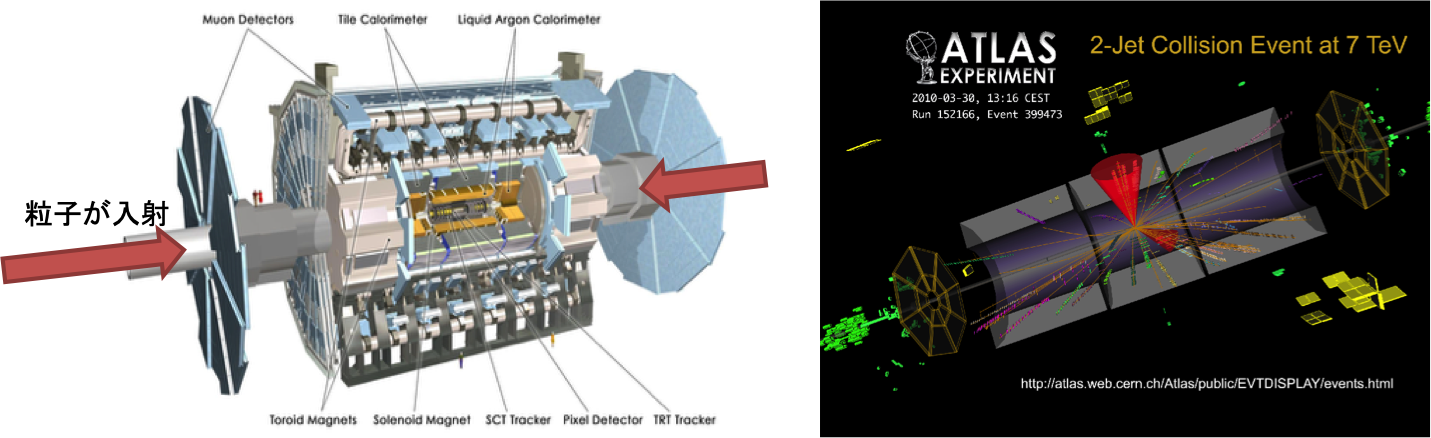
\includegraphics[width=15cm]{./atlas.png}
\caption{検出器の外観と粒子の入射方向}
\end{center}
\end{figure}

%\subsubsection{LHC-ATLAS実験}
%加速器は、1930年代い原子核の構造を調べるために発明されて以来、粒子物理学の様々な発見に貢献してきた。加速器には線形のものと円形のものとがあり、LHCは円形の加速器である。LHC-ATLAS実験では、加速した陽子同士を高エネルギーで正面衝突させて陽子の構成要素であるクォークやグルーオンといった素粒子が散乱する様子を観測する。陽子は電子よりも質量が大きい(約1840倍)ため、シンクロトロン放射によるエネルギー損失が小さく、円形で徐々に加速して高エネルギーの粒子を得ることができる。

\subsubsection{粒子識別}
粒子を識別するためには、電磁力を用いて、比較的安定な粒子を検出する。粒子識別に必要な測定すべき運動量は
\begin{itemize}
\item エネルギー$\vec{E}$
\item 運動量$\vec{p}$
\item 速度$\vec{v}$
\item 質量$M$
\end{itemize}
以上のうちの2つである。\\
また測定する方法としては、
\begin{itemize}
\item 電磁力で曲げて運動量$\vec{p}$を測る
\item エネルギーを$\vec{E}$吸収させて測る
\item 通過時間で測る
\item 不変質量や既知の質量を用いる
\end {itemize}
がある。今回は、「電磁力で曲げて運動量$\vec{p}$を測る」方法について、説明する。

\subsubsection{曲げて測る}
検出器の外観と、粒子が入射する方向は以下のようになっている。

また、磁場は以下のようにかかっている。
\begin{figure}[h]
\begin{center}
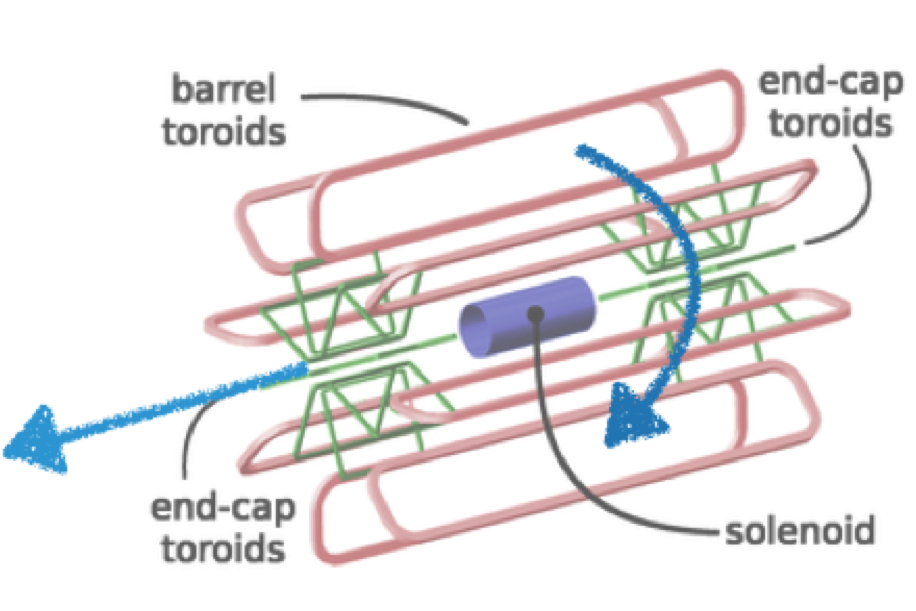
\includegraphics[width=6cm]{./magne.png}
\caption{磁場のかかる方向}
\end{center}
\end{figure}

このように磁場をかけることで、運動量$\vec{p}$を測ることが可能になる。\\
\begin{figure}[h]
\begin{center}
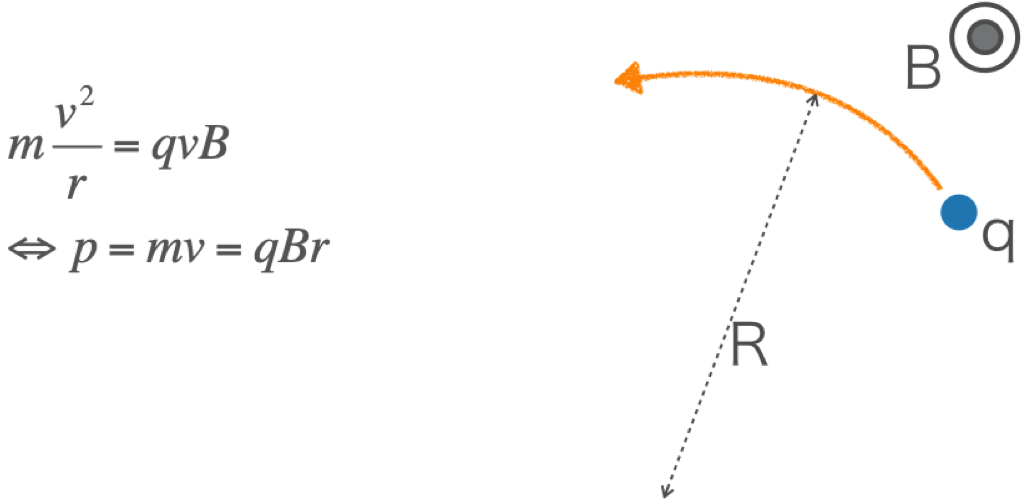
\includegraphics[width=10cm]{./circle.png}
%\caption{粒子の円運動}
\end{center}
\end{figure}
磁場中で円運動をすることで、以下の式のように半径から運動量を求めることができる。\\
このようにして、粒子識別のために必要な物理量の1つである運動量を測定することができる。

\end{document}


